\documentclass[a4paper,12pt]{article}

\usepackage{graphicx} % Required for inserting images
\usepackage{amsmath,amssymb,amsfonts}
\usepackage{subcaption}
% -----------------------
% Package Imports
% -----------------------

% Set page margins
\usepackage[a4paper, top=1in, bottom=0.8in, left=1.1in, right=0.8in]{geometry}

% Use Times New Roman font
\usepackage{times}





% Set page margins
\usepackage[a4paper, top=1in, bottom=0.8in, left=1.1in, right=0.8in]{geometry}


% Add page numbering
\pagestyle{plain}

% Enable graphics inclusion
\usepackage{graphicx}
\usepackage{float}
% Enable code listings
\usepackage{listings}
\usepackage{xcolor} % For customizing code colors
\setlength{\parindent}{0pt}
\usepackage{multirow}

\setlength{\parindent}{0pt}
\usepackage{titlesec} % To customize section font size
\titleformat{\section}
{\normalfont\fontsize{14}{16}\bfseries}{\thesection}{1em}{}

\titleformat{\subsection}
{\normalfont\fontsize{14}{16}\bfseries}{\thesubsection}{1em}{}

\begin{document}
	\section{Experiment No. 8}
	
	\section{Experiment Title }
Starting of Single-Phase Induction Motor by Capacitor.
	
	\section{Objective}
	
	The objectives of this lab are as follows:
	\begin{itemize}
		\item 	To understand the need for a starting mechanism in a single-phase induction motor due to its non-self-starting nature.
		\item 	To study the role of a capacitor in creating a phase difference between the main and auxiliary windings for generating starting torque.
		
		\item  To observe the starting performance of a single-phase induction motor with and without a capacitor.
		
		
	\end{itemize}
	\section{Theory}
	
	A single-phase induction motor is an AC motor that operates on a single-phase power supply, such as typical household electricity. It is commonly used in small appliances including fans, blowers, washing machines, and water pumps.
	
	Unlike three-phase motors, a single-phase induction motor has only one stator winding, known as the \textit{main winding}. When connected to an AC supply, this winding produces a \textbf{pulsating magnetic field}—one that alternates in magnitude but does not rotate. As a result, the motor is not self-starting because there is no rotating magnetic field at startup to produce initial torque. This situation can be summarized as follows:
	
	\begin{itemize}
		\item The magnetic field oscillates back and forth but does not rotate.
		\item Consequently, the rotor either remains stationary or only vibrates without initiating rotation.
	\end{itemize}
	
	To make the motor self-starting, an \textbf{auxiliary winding} (also called a \textit{starting winding}) is added. This winding is placed 90$^\circ$ electrically apart from the main winding. A capacitor is connected in series with the auxiliary winding to introduce a phase shift between the currents in the two windings. This phase difference creates a \textbf{rotating magnetic field}, which is necessary to generate starting torque.
	
	The expression for the starting torque \(\tau\) is given by:
	
	$$
	\tau \propto V^2 \sin(2\theta)
	$$
	
	Where:
	\begin{itemize}
		\item \(V\) = voltage applied to the windings
		\item \(\theta\) = phase angle between the currents in the main and auxiliary windings
	\end{itemize}
	
	\subsection*{Role of the Capacitor in Starting}
	
	\begin{itemize}
		\item The capacitor introduces an approximate 90$^\circ$ phase shift between the main and auxiliary winding currents.
		\item This phase difference effectively creates a two-phase rotating magnetic field, similar to that in a three-phase motor, which enables self-starting behavior.
	\end{itemize}
	
	After the motor reaches about 70--80\% of its rated speed, a centrifugal switch or relay disconnects the auxiliary winding to prevent excessive current and overheating. Additionally, the presence of the capacitor results in smoother operation, higher starting torque, and quieter performance compared to split-phase motors without capacitors.
	
	Thus, the capacitor-start method overcomes the non-self-starting limitation of single-phase induction motors by creating an artificial two-phase supp
	
	\section{Circuit Diagram}
	\begin{figure}[H]
		\centering
	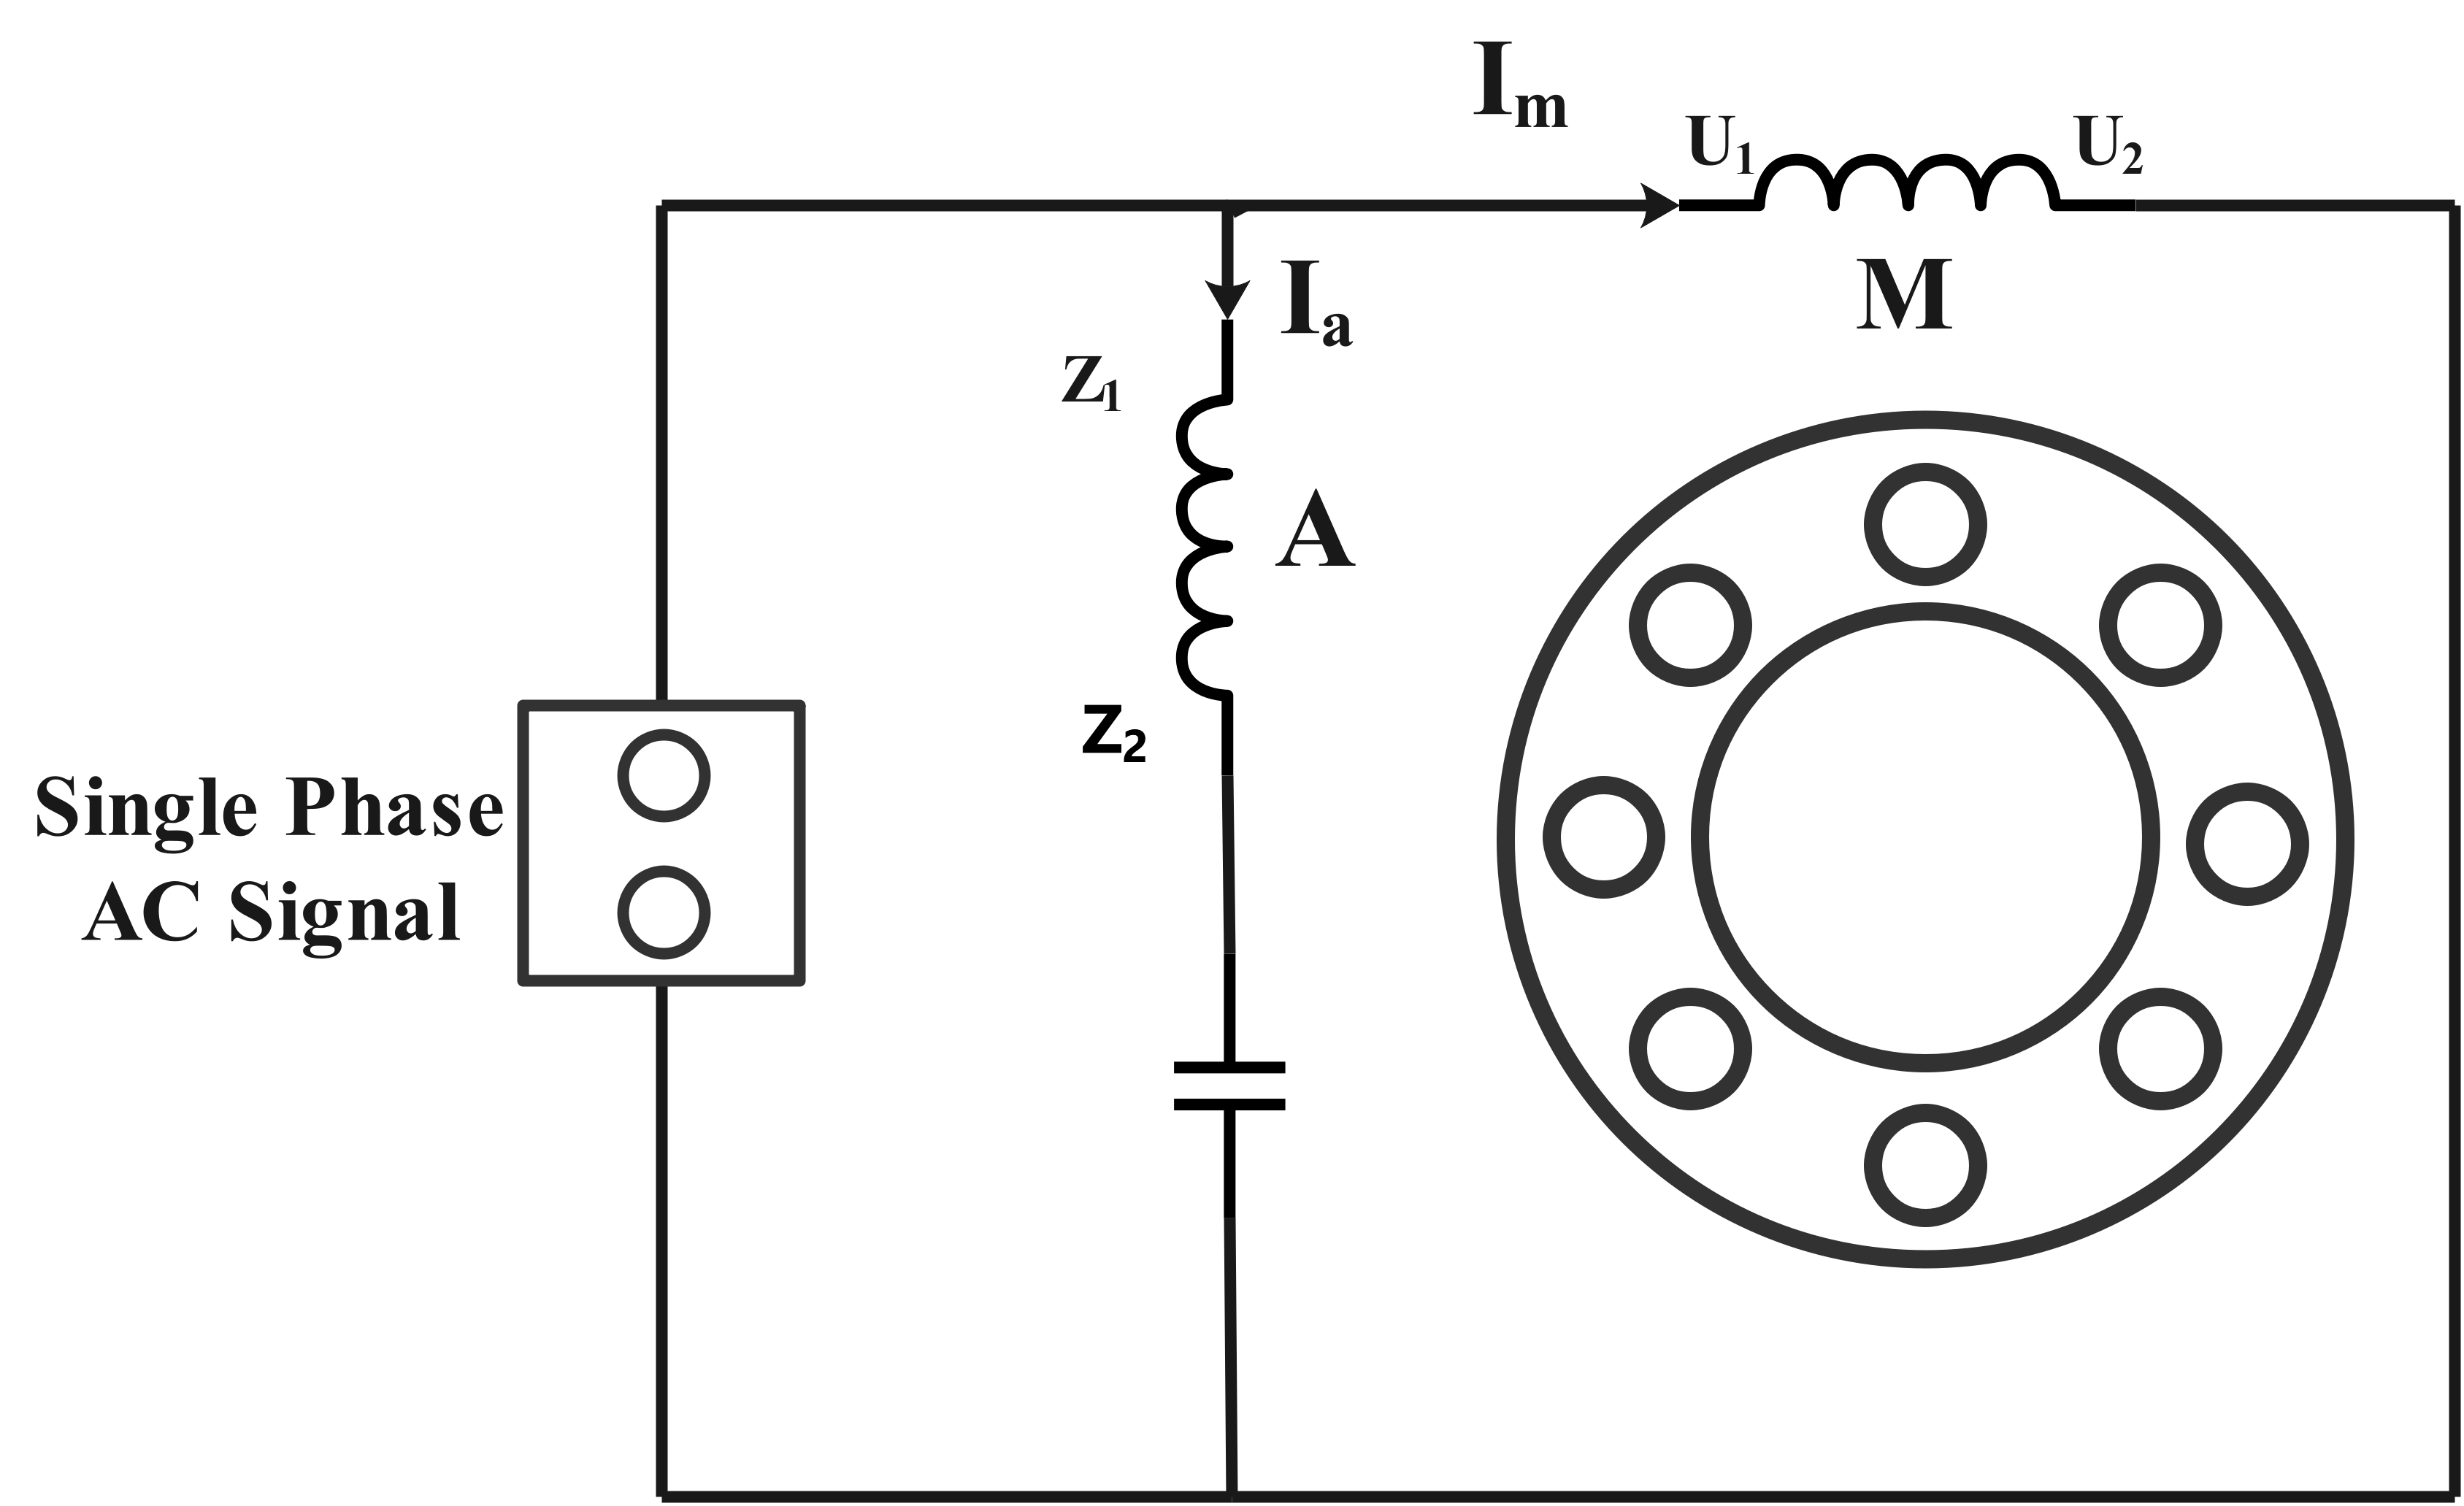
\includegraphics[width=0.7\textwidth]{Images/1}
		\caption{Capacitor run single phase Induction Motor}
		
	\end{figure}
	
	
	
	
	\section{Required Apparatus}
	
	\begin{enumerate}
		\item \textbf{Single-Phase Induction Motor}
		\begin{enumerate}
			\item Maximum Current: \( I_{\text{max}} = 3.7\,\text{A} \)
			\item Maximum Speed: \( \text{Speed}_{\text{max}} = 2700\,\text{rpm} \)
			\item Maximum Voltage: \( V_{\text{max}} = 230\,\text{V} \)
		\end{enumerate}
		
		\item \textbf{AC Power Supply}
		\begin{enumerate}
			\item Voltage Range: \( V = 0 - 230\,\text{V} \)
		\end{enumerate}
		
		\item \textbf{3-Phase Meter}
		\begin{enumerate}
			\item Voltage: \( 500\,\text{V}_{\text{rms}} \)
			\item Maximum Current: \( 5\,\text{A} \)
		\end{enumerate}
		
		\item \textbf{Connecting Wires}
		\begin{enumerate}
			\item No additional parameters
		\end{enumerate}
	\end{enumerate}
	
	\section{Observation}
	\begin{table}[H]
		\centering
		\begin{tabular}{|c|p{12cm}|}
			\hline
			\textbf{Case} & \textbf{Observation} \\
			\hline
			1 & Using only the primary winding, the motor did not start at any voltage, even when manually rotated. \\
			\hline
			2 & Using only the auxiliary winding, the motor also failed to start; no startup or torque generation was observed. \\
			\hline
			3 & Using both primary and auxiliary windings without a capacitor, the motor started only when manually rotated at a steady speed. \\
			\hline
			4 & Using both windings with a capacitor, the motor started automatically at 50.6 V due to the double revolving magnetic flux. \\
			\hline
			5 & After starting the motor with both windings and a capacitor, it continued rotating even after the capacitor was disconnected during running condition. \\
			\hline
			\multicolumn{2}{|l|}{\textbf{Additional Observations}} \\
			\hline
			\multicolumn{2}{|l|}{• At half of the rated voltage, the motor ran smoothly.} \\
			\multicolumn{2}{|l|}{• At full rated voltage, the motor vibrated.} \\
			\hline
		\end{tabular}
		\caption{Observations of Motor Behavior under Different Conditions}
	\end{table}
	

	\section{Discussion}
	
	In this experiment, the behavior of a single-phase induction motor was observed under five different conditions to understand its starting characteristics and performance.It was found that the motor could not start when only the primary or auxiliary winding was used individually (Cases 1 and 2).In Case 3, when both the primary and auxiliary windings were connected without a capacitor, the motor started only with manual assistance.When a capacitor was introduced in Case 4, automatic startup was achieved at a voltage of 50.6 V. This demonstrated that the required phase shift created by the capacitor generated a rotating magnetic field, providing the necessary starting torque.In Case 5, it was observed that the motor continued running smoothly even after the capacitor was disconnected once full speed was reached. 
	

	
	Overall, the experiment effectively demonstrated the critical role of the auxiliary winding and capacitor in enabling self-starting in single-phase induction motors.
	
	

	
\end{document}
